% ----------------------------------------------------------------------

\newpage

\subsection{\bb Test}
\label{ss:bb}

\subsubsection{Purpose}

The \bb test is meant to flag any problems with the bump bonds that connect the sensor to the ROCs
and form the path for the charge generated in the silicon sensor to be recorded by the ROCs.
This test takes advantage of a parallel route designed for the calibration signal in the ROC.
This route can be seen at the top left of Figure~\ref{fig:puc}, 
connecting the source of the \vcal calibration pulse to the ``top metal pad'' 
by closing the switch labelled ``sensor calib'' instead of the standard ``calib'' switch.
The ``top metal pad'' is on near the top edge of the \roc on the side facing the sensor.
The calibration pulse can pass via capacitive coupling from this pad, 
across the \roc-sensor air gap, into the silicon sensor.
The calibration pulse then makes its way back into the \roc via the bump bond and can be read out as normal.
Using this signal path that contains the bump bond, 
the presence of the bump and the quality of its electrical connection from the sensor to the \roc can be tested.

Currently in pXar there are four variants of bump bonding tests, optimized to different module types.  
For FPix modules, the standard test is the {\tt BB3} test.
This document focuses on this specific \bb test version.

\subsubsection{\textcolor{red}{Methodology}}



\subsubsection{Output}

\begin{figure}[!Hp]
\centering
\begin{minipage}{0.45\textwidth}
  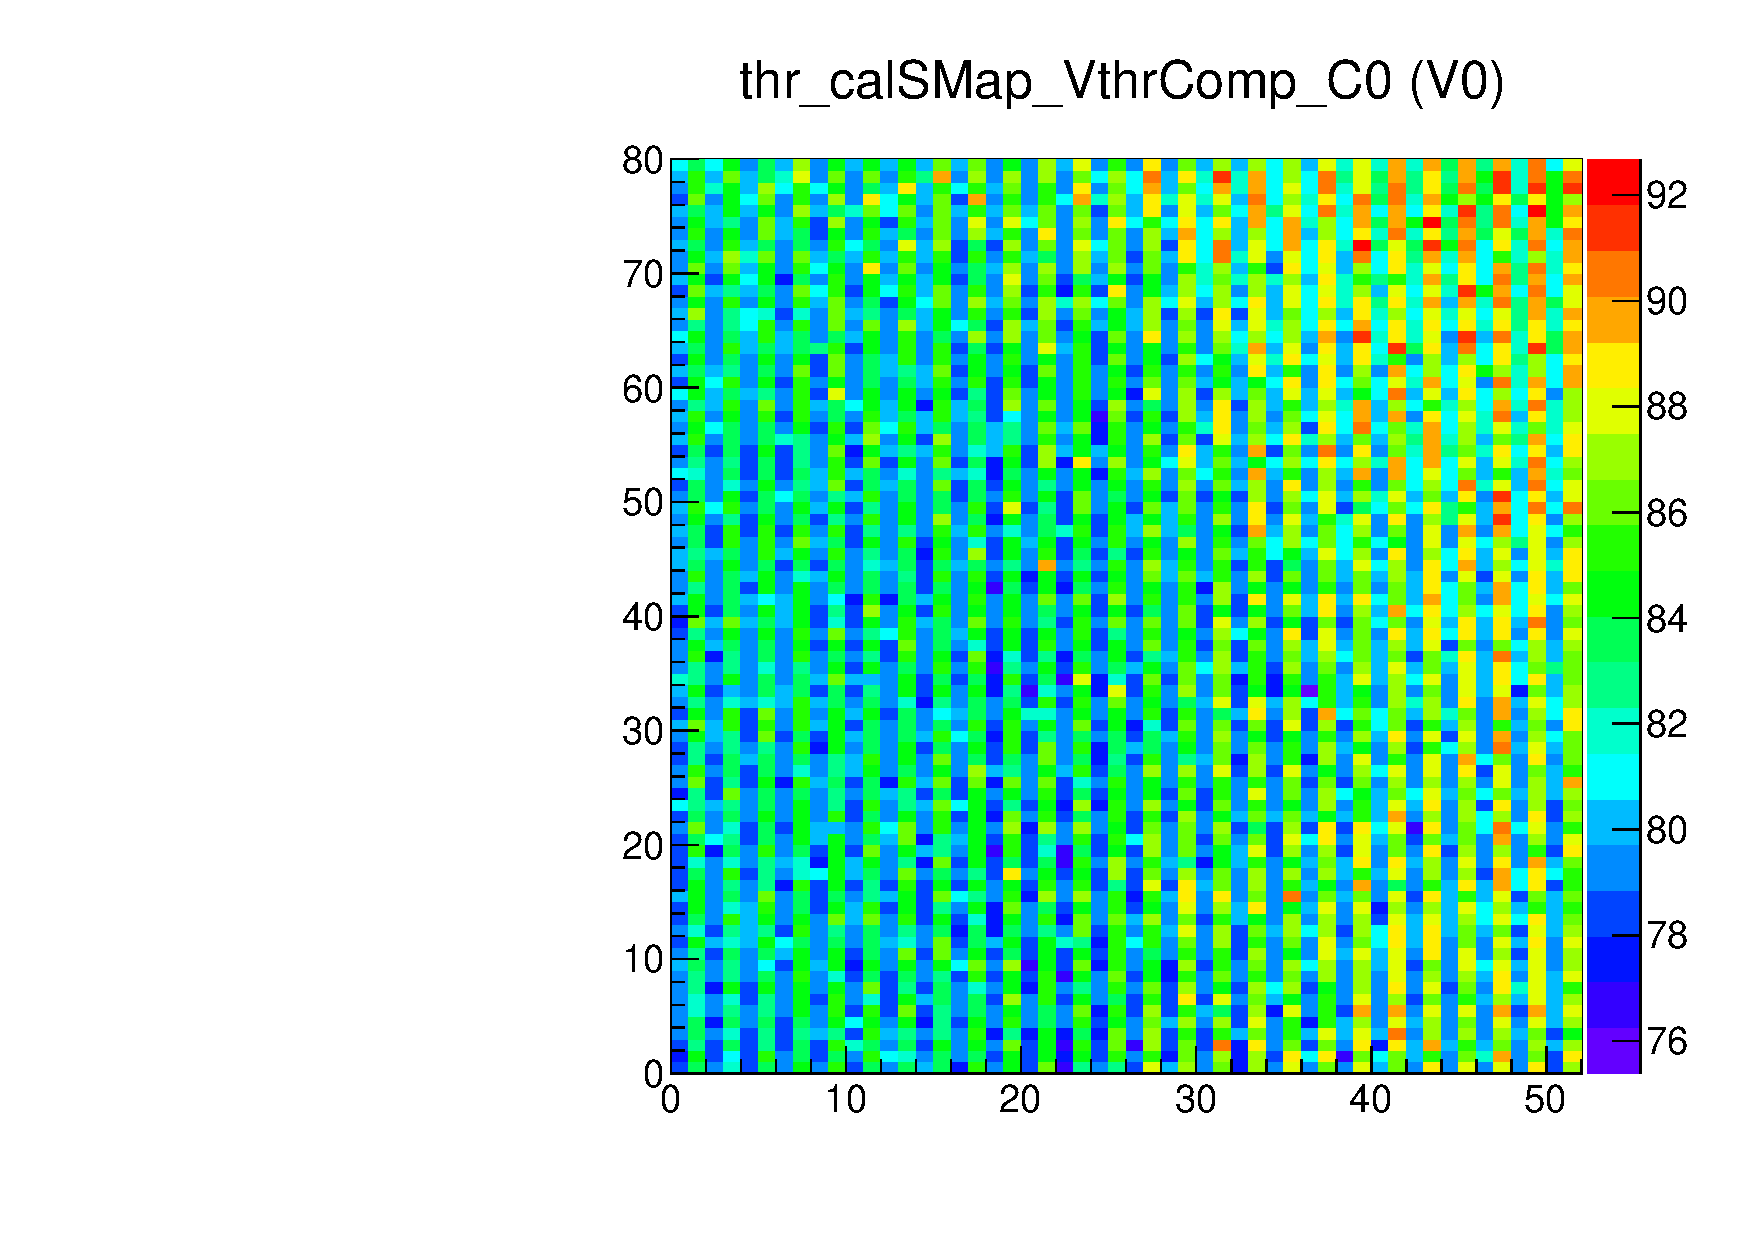
\includegraphics[width=1.0\textwidth]{figures/bb3_thr_calSMap_VthrComp.pdf}
  \caption{\roc map of the raw \vthrcomp turn-on values when passing the calibration pulse through the sensor.}
  \label{fig:bb3_thr_calSMap_VthrComp}
\end{minipage}
\end{figure}

\begin{figure}[!Hp]
\centering
\begin{minipage}{0.45\textwidth}
  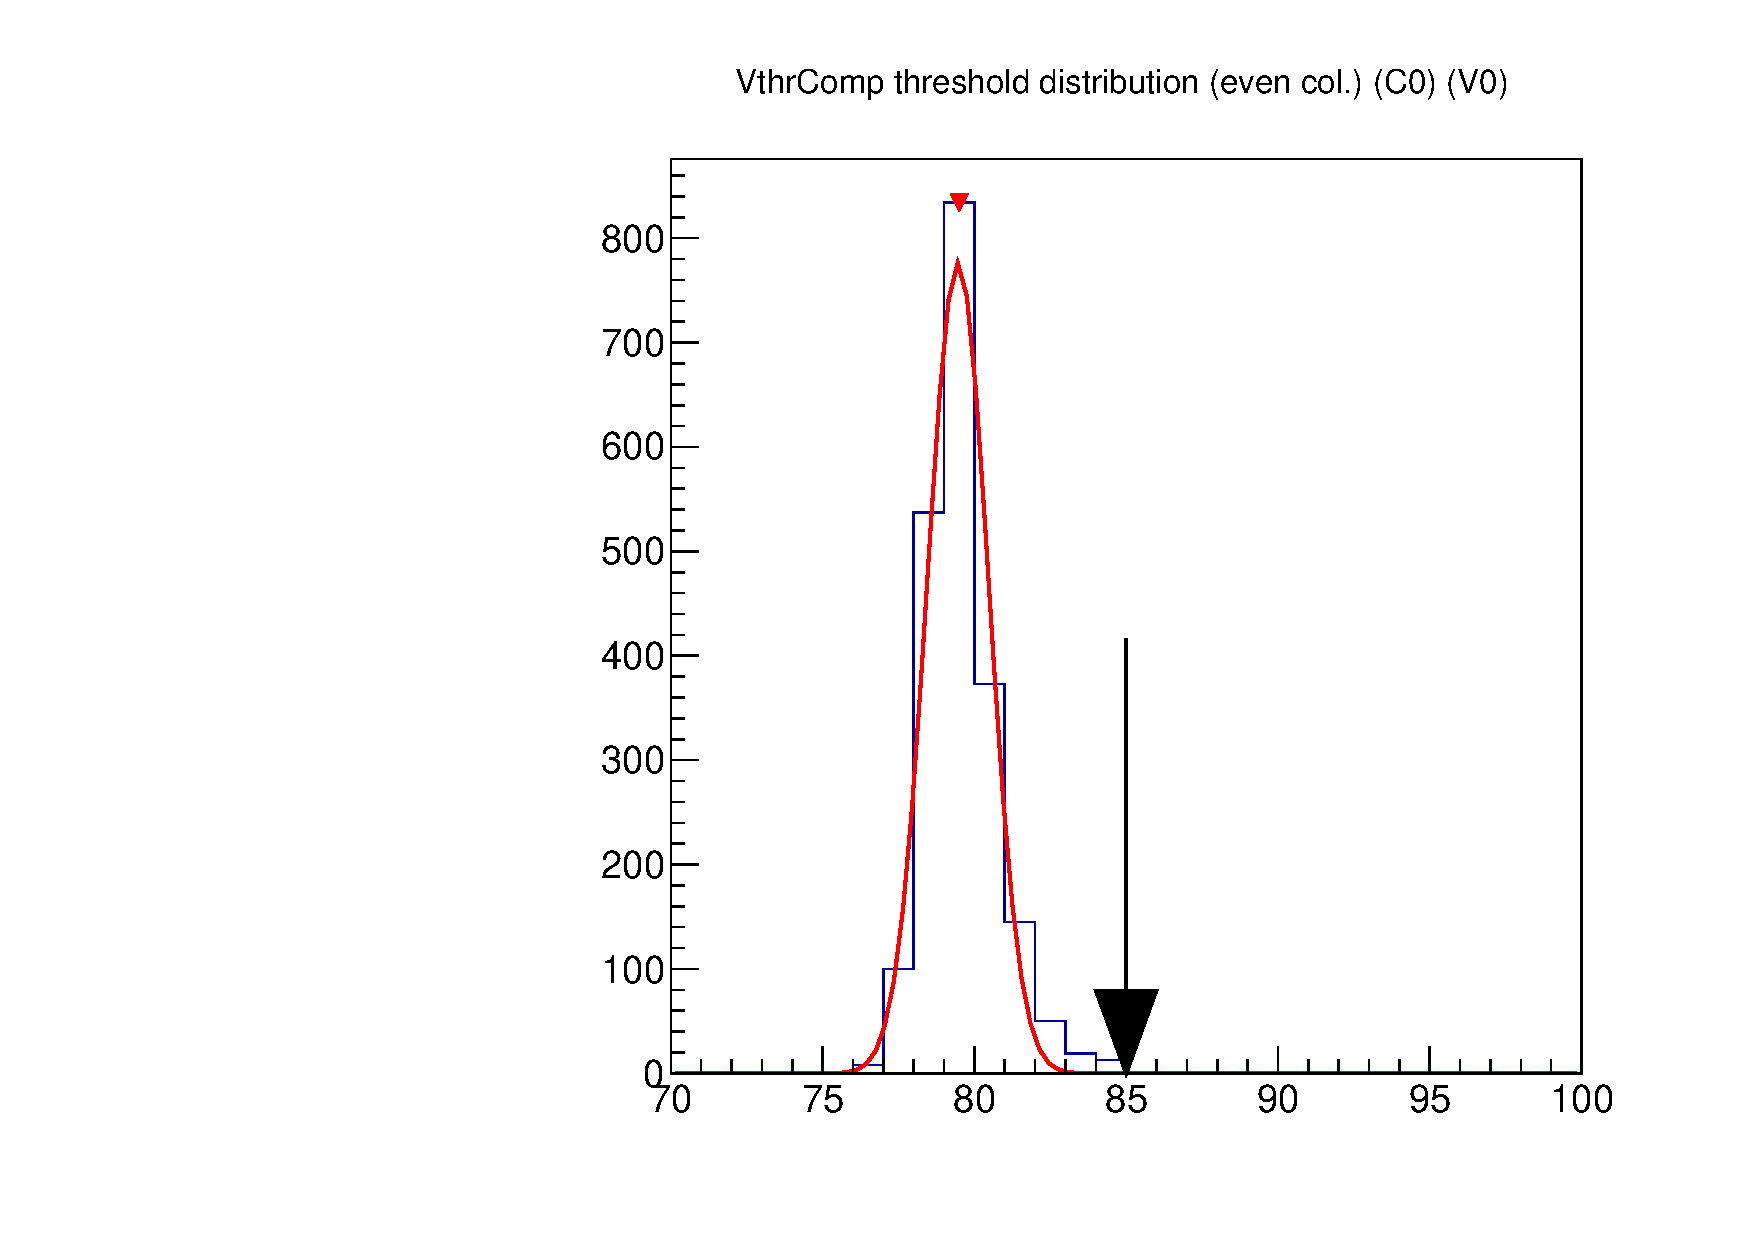
\includegraphics[width=1.0\textwidth]{figures/bb3_dist_thr_calSMap_VthrComp_EvenCol.pdf}
  \caption{1D distribution of the even columns in Figure~\ref{fig:bb3_thr_calSMap_VthrComp}.
  The red curve is a Gaussian fit to the data.
  The black arrow corresponds to 5$\sigma$ above the fitted peak.
  [original range 0-255]}
  \label{fig:bb3_dist_thr_calSMap_VthrComp_EvenCol}
\end{minipage}
\hspace{0.3cm}
\begin{minipage}{0.45\textwidth}
  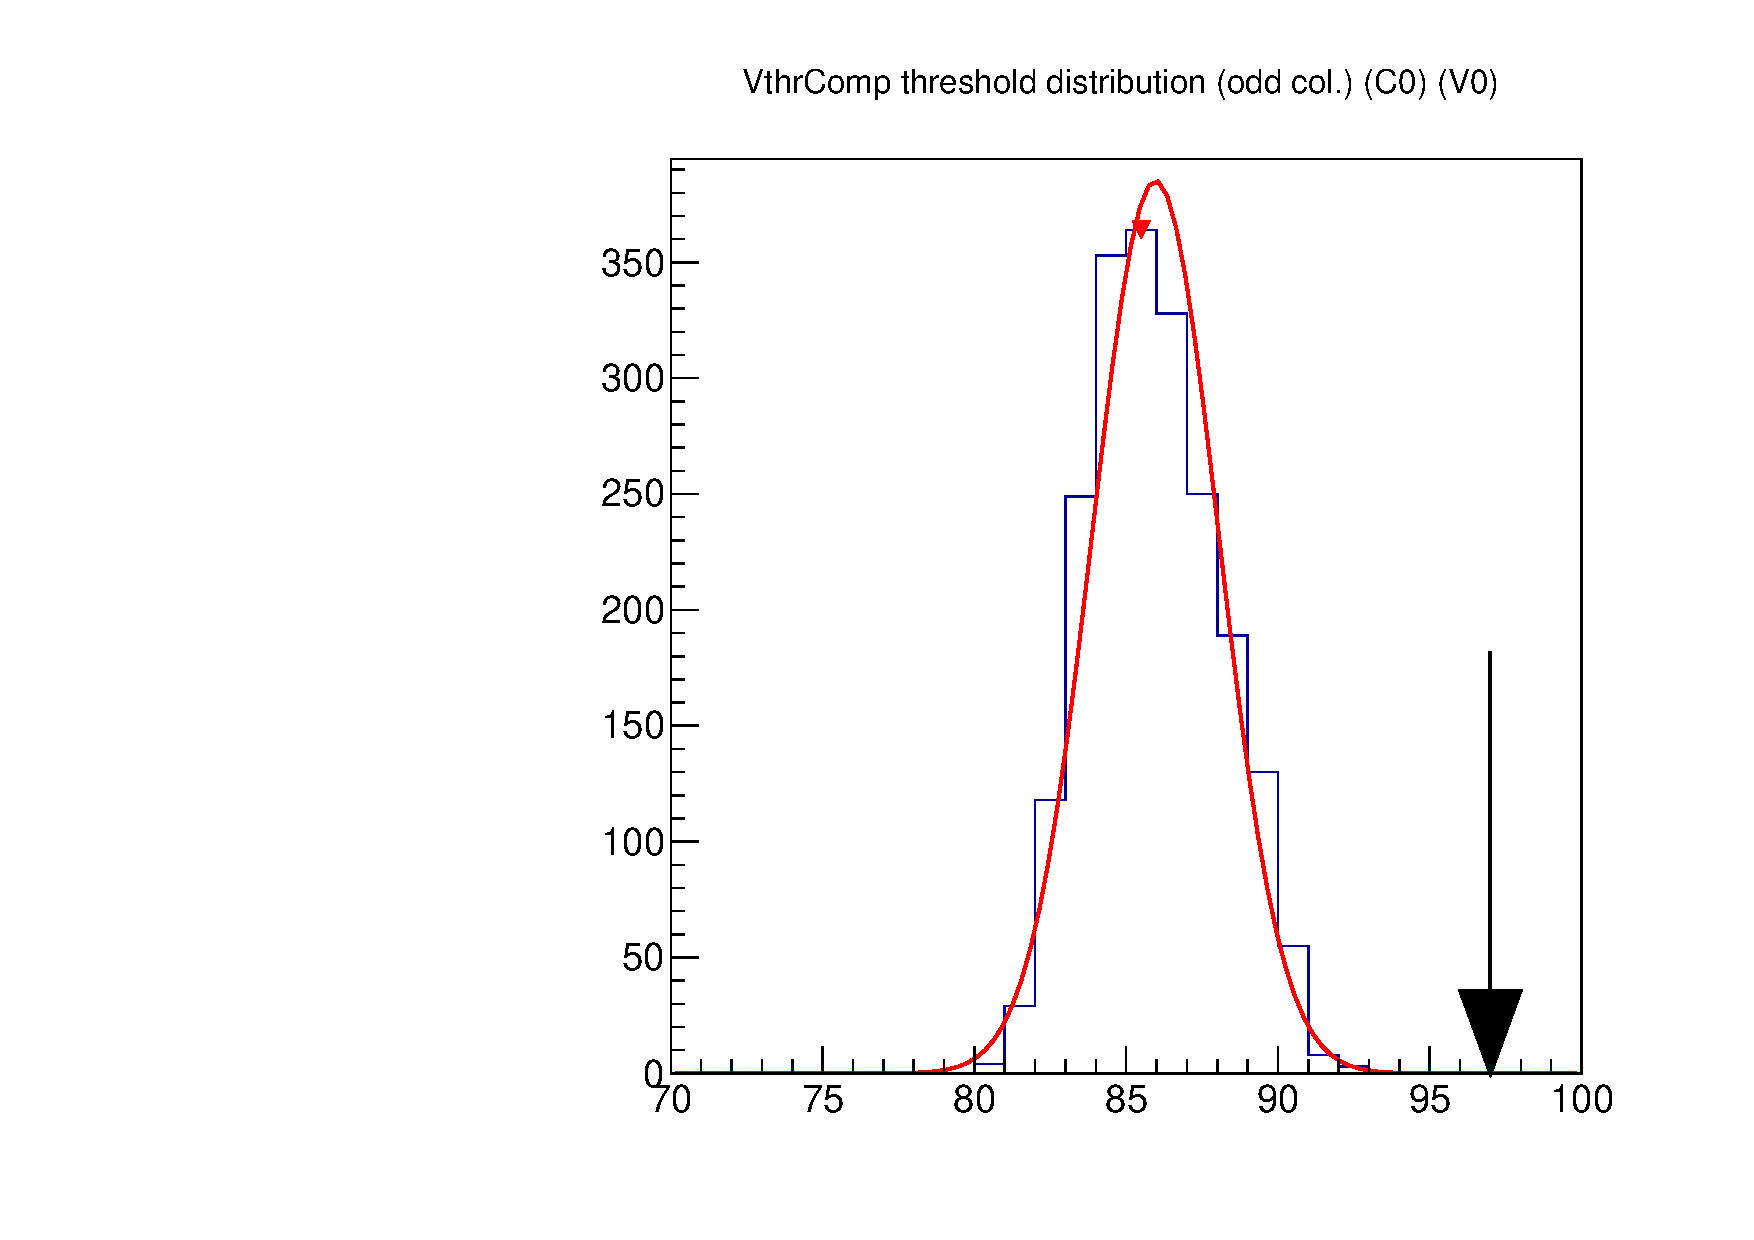
\includegraphics[width=1.0\textwidth]{figures/bb3_dist_thr_calSMap_VthrComp_OddCol.pdf}
  \caption{1D distribution of the odd columns in Figure~\ref{fig:bb3_thr_calSMap_VthrComp}.
  The red curve is a Gaussian fit to the data.
  The black arrow corresponds to 5$\sigma$ above the fitted peak.
  [original range 0-255]}
  \label{fig:bb3_dist_thr_calSMap_VthrComp_OddCol}
\end{minipage}
\end{figure}

\begin{figure}[!Hp]
\centering
\begin{minipage}{0.45\textwidth}
  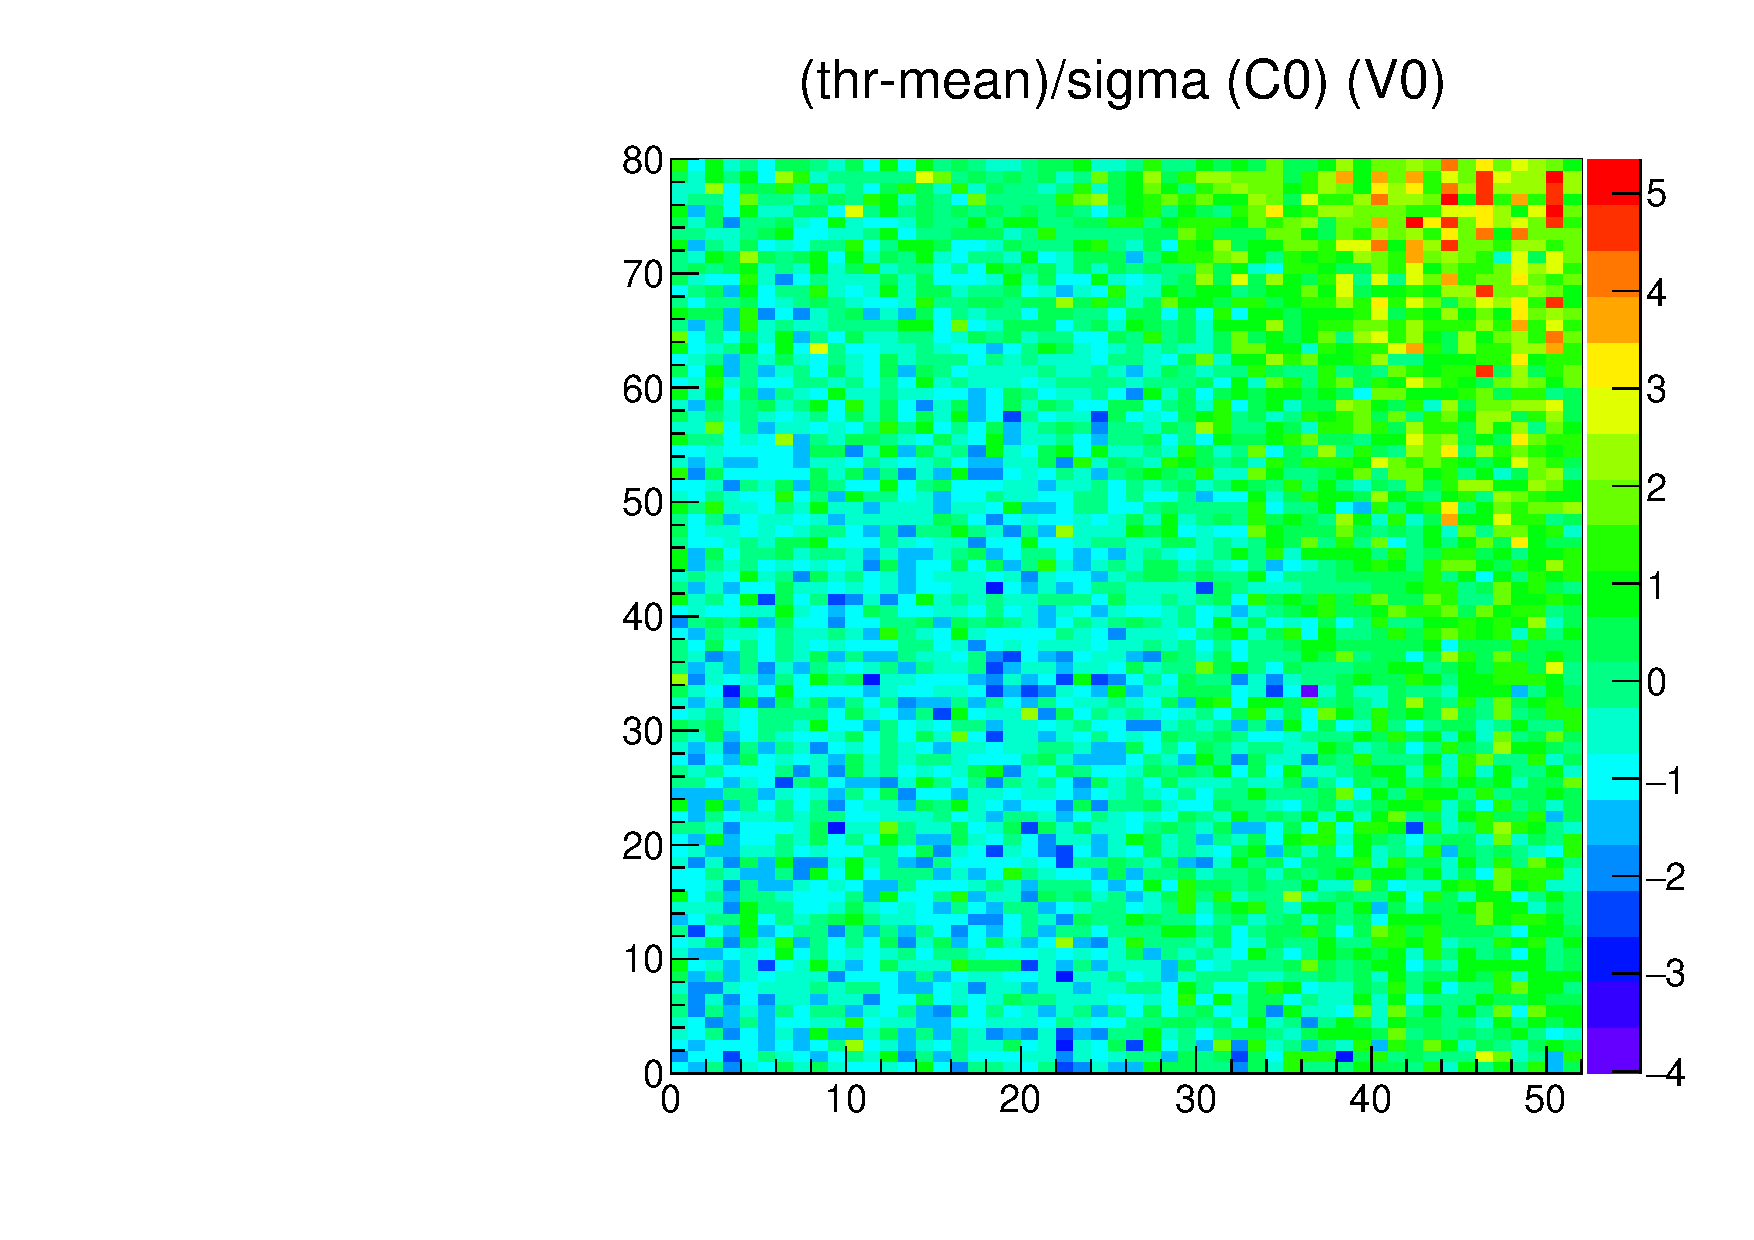
\includegraphics[width=1.0\textwidth]{figures/bb3_rescaledThr.pdf}
  \caption{\roc map of the residuals of the \vthrcomp turn-on values, 
  calculated separately for even and odd columns.}
  \label{fig:bb3_rescaledThr}
\end{minipage}
\hspace{0.3cm}
\begin{minipage}{0.45\textwidth}
  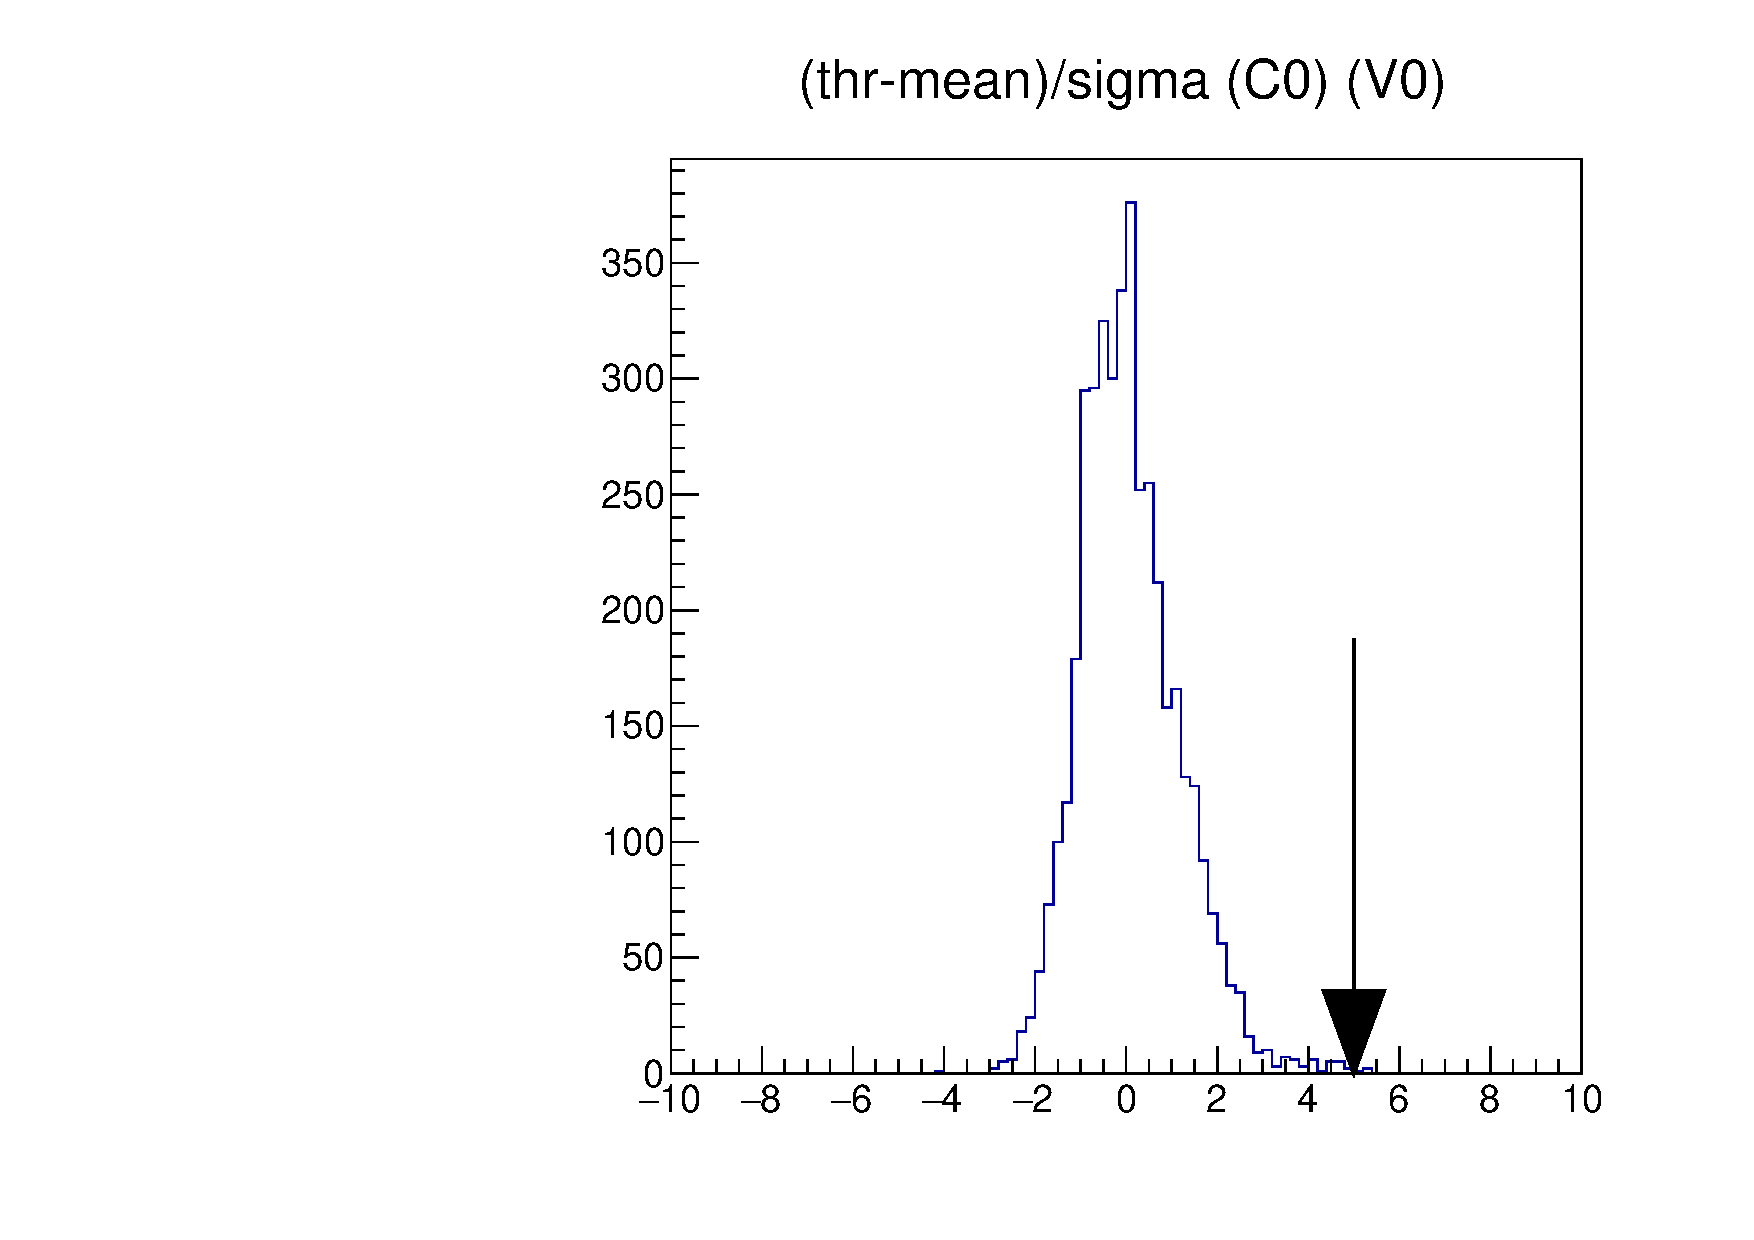
\includegraphics[width=1.0\textwidth]{figures/bb3_dist_rescaledThr.pdf}
  \caption{1D distribution of \roc map in Figure~\ref{fig:bb3_rescaledThr}.
  Pixels with turn-on values more than 5$\sigma$ above the \roc mean 
  (marked by the black arrow) are flagged as faulty.}
  \label{fig:bb3_dist_rescaledThr}
\end{minipage}
\end{figure}

